\documentclass[12pt, a4paper, lithuanian]{article}
\usepackage[utf8x]{inputenc}
\def\LTfontencoding{L7x}
\PrerenderUnicode{ąčęėįšųūž}
\usepackage[\LTfontencoding]{fontenc}
\usepackage[lithuanian]{babel}
\usepackage{VUMIFPSkursinis}
\usepackage{cite}
\usepackage{amsmath}
\usepackage{bm}
\usepackage{amsfonts}
\usepackage{float}
\usepackage{graphicx}
\usepackage{color}
\usepackage{listings}
\usepackage{wrapfig}
\usepackage{algpseudocode}
\usepackage{algorithm}
\usepackage{algorithmicx}
\usepackage{caption}
\usepackage{subfig}


% Titulinio aprašas
\vumifdept{Programų sistemų katedra}
\vumifpaper{Kursinis darbas}
\title{Biojutiklio su selektyvia membrana kompiuterinis modeliavimas}
% \title{Esama situacija su dviem sluoksniais}
% \title{Ištirti selektyvios membranos įtaką amperometrinio biojutiklio jautriui}
\def\titleineng{Computational modelling of biosensors with selective membrane}
\def\statusas{% Kai kurioms katedroms reikia nurodyti  
    4 kurso 1 grupės studentas \\
}
\author{
   Kęstutis Gimbutas
}

\supervisor{prof. dr. Romas Baronas}
\date{Vilnius – \the\year}

\begin{document}
\sloppy
\maketitle

\tableofcontents

\sectionnonum{Įvadas}
Biojutikliai yra analitiniai prietaisai, kurių pagrindinės sudedamosios dalys
yra biologinis darinys, kuris atpažįsta norimus cheminius junginius, ir
prietaisas, kuris to junginio atpažinimą  paverčia į elektros signalą \cite{baronas2009mathematical}. Elektros
signalo stiprumas yra proporcingas minėto cheminio elemento koncentracijai
nagrinėjamoje terpėje. Biojutikliai yra klasifikuojamini pagal įrenginio, kuris
paverčia vienos rūšies energiją kita,
prigimtį. Amperometriniai biojutikliai matuoja srovės stiprį faradais, kuri
kyla elektrode dėl biocheminės reakcijos produktų tiesioginės cheminės oksidacijos 
arba redukcijos. Kol matuojama srovė amperometriniuose biojutikliuose elektrodo potencialas yra
laikomas konstanta. Amperometriniai biojutikliai yra žinomi
kaip patikimi, pigūs ir reikšmingi medicinos, pramonės sritims.

Praktiškas biojutiklis turi daugiasluoksnę fermento membraną. Elekrodas veikia
kaip biojutiklio rėlė, jis yra padengtas selektyviaja membrana po kurios seka
imobilizuotas fermentas. Selektyvioji membrana yra naudojama norint padidinti
biojutiklio selektyvumą \cite{baronas2006computational}.

Šiame darbe yra remiamasi \cite{baronas2009mathematical} knygos 44-56psl.
aprašytomis amperometrinių biojutiklių, kurių pagrindinės sudedamosios dalys
yra elektrodas ir fermento sluoksnis, charakteristikomis. Joms bus adaptuota
selektyvioji membrana: sudarytas amperometrinio biojutiklio su selektyvia
membrana matematinis modelis, sumodeliuotos jo atsako charakteristikos, bus
išvestas biojutiklio matematinio modelio skaitinės aproksimacijos ir atlikta
biojutiklios veikimo simuliacija naudojantis parašyta programa.

Tai įgyvendinus bus galima tirti selektyvios membranos įtaką biojutiklio
atsakui, apskaičiuoti optimalų selektyvios membranos arba fermento sluoksnio
storį žinant vieną iš jų ir difuzinius koeficientus bei tobulinti suformuotą
amperometrinio biojutiklio su selektyvia membrana modelį papildant jį naujais
scenarijais ir sąlygomis.

\section{Biojutiklio su selektyvia membrana modelis}
%Sudarant modelius bei lygtis buvo pasinaudota šaltiniais:
%\cite{baronas2009mathematical}, \cite{baronas2006computational},
%\cite{baronas2003influence}.

\subsection{Matematinis modelis}

Supaprastintas amperometrinis biojutiklis su seletyvia membrana turi tris
pagrindines sudedamąsias dalis: fermento sluoksnis($\Omega_2$),
selektyvios
membranos sluoksnis($\Omega_1$), elektrodas (žr. 1 pav.).
\begin{figure}[H]
    \centering
    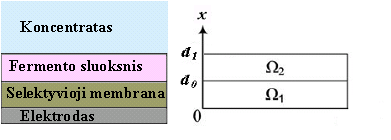
\includegraphics[scale=0.9]{img/modv1}
    \caption{Biojutiklio struktūra}
    \label{biojutiklio-struktura}
\end{figure}

Fermento sluoksnyje vyksta grįžtamoji cheminė reakcija, kurios metu (S)
, kuris supa biojutiklį,
susijungia su (E), kad suformuotų kompleksą (ES). Susiformavus minėtam
kompleksui jis pasidalija į reakcijos produktą (P) ir fermentą (E)
\cite{baronas2009mathematical}.  
\begin{equation}
    S + E \leftrightarrow ES \rightarrow E + P
\end{equation}

Selektyvios membranos sluoksnis yra skirtas atskirti (P) iš fermento sluoksnyje esančių
junginių. Dažniausiai tam yra naudojamos kietesnės ir didesnio tankio medžiagos
nei fermento sluoksnis, todėl selektyvios membranos ir (P) difuzinis
koeficientas yra mažesnis lyginant su (E) ir (S) arba (E) ir (P) difuziniais
koeficientais. Taip pat šis sluoksnis gali pagerinti kitas biojutiklio savybes kaip
tvirtumas, elektrodo ilgaamžiškumas. 

Junginiui (P) difuzijos būdu nukeliavus iki elektrodo įvyksta cheminė reakcija,
kurios pasakoje junginys (P) yra visiškai suvartojamas ir elektrode susidaro
elektros srovė. Daroma prielaida, kad šios reakcijos metu nesusidaro šalutiniai
produktai ir elektrodas nesidėvi.

Remiantis supaprastinta schema substratas (S) prisijungia prie fermento (E)
ir yra
paverčiamas į produktą (P),
\begin{equation}\label{eq:basic}
    S \overset{E}{\rightarrow} P
\end{equation}

Biojutiklio veikimo simuliacija bus modeliuojama vienoje erdvės dimensijoje,
todėl sritys apibrėžiamos intervaluose. Uždaros sritys, kurios atitinka fermento ir selektyvios
membranos sluoksnius, atvaizduotos \ref{biojutiklio-struktura} pav.:
\begin{equation}
\begin{aligned}
    &\overline{\Omega}_1 = [0, d_0],\\
    &\overline{\Omega}_2 = [d_0, d_1]
\end{aligned}
\end{equation}

Tegu $\Omega_i$ yra atviros sritys atitinkančios uždarus regionus
$\overline{\Omega}_i$, $i = 1, 2$:
\begin{equation}
\begin{aligned}
    &\Omega_1 = (0, d_0),\\
    &\Omega_2 = (d_0, d_1)
\end{aligned}
\end{equation}

Srityje $\Omega_1$ vyksta tik produkto, tuo tarpu $\Omega_2$ srityje vyksta fermento
reakcija su substratu ir jų transportavimas difuzija.

Apjungus fermento katalizuojamą reakciją fermento sluoksnyje su reakcijos
produkto (P) difuzija selektyviojoje membranoje ir su vienos
dimensijos erdvėje difuzija, kuri yra apibrėžta Ficko dėsniu, gautos šios
esminės lygtys:
\begin{equation}
\begin{aligned} 
    \label{eq:mat-modelis}
    &\frac{\partial P_1}{\partial t} = D_{1P} \frac{\partial^2 P_1}{\partial x^2}, \;
    \; x \in \Omega_1,\\
    &\frac{\partial S}{\partial t} = D_S \frac{\partial^2 S}{\partial x^2} -
    \frac{V_{max} S}{K_M + S},  \\ 
    &\frac{\partial P_2}{\partial t} = D_{2P} \frac{\partial^2 P_2}{\partial x^2} +
    \frac{V_{max} S}{K_M + S}, \; \; x \in \Omega_2 ,\;\; t > 0.\\
\end{aligned}
\end{equation}

Lygčių sistemoje (\ref{eq:mat-modelis}) $x$ atitinka erdvę, o $t$ – laiką, $S(x, t)$
yra substrato koncentracija, o $P(x, t)$ yra reakcijos produkto koncentracija,
$\Omega_1$ – selektyvios membranos storis, $\Omega_2$ – fermento sluoksnio
storis, $V_{max}$ – maksimalus fermentacinis greitis, $ D_{1P}$, $ D_{2P}$, $ D_S$ - difuziniai medžiagų koeficientai, t - laikas nuo
simuliacijos pradžios, $ K_M$ - Michaelio konstanta. Michaelio konstanta $K_M$
nusako su kokios koncentracijos substratu yra pasiekiama pusė maksimalaus
reakcijos, kuri katalizuojama fermento, greičio.

\subsection{Pradinės ir kraštinės sąlygos}
Tegu $x = 0$ yra elektrodo paviršius, $x = d_1$ – riba tarp analizuojamo
substrato ir fermento membranos, o $x = d_0$ – riba tarp selektyviosios membranos
ir fermento sluoksnio. Iš pradžių nei (S) nei (P) nėra biojutiklio
dalyse. Matavimai pradedami, kai substratas atsiduria ant fermento membranos
paviršiuje. Pradinėmis sąlygomis ($t = 0$) tikimasi:
\begin{equation}
\begin{aligned}
    &S(0,0) = 0, \\
    &S(x, 0) = 0,\; x \in \Omega_2,\\
    &S(d_1, 0) = S_0,
\end{aligned}
\end{equation}

\begin{equation}
\begin{aligned}
    &P_1(x, 0) = 0,\; x \in \overline\Omega_1,\\
\end{aligned}
\end{equation}

\begin{equation}
\begin{aligned}
    &P_2(x, 0) = 0,\; x \in \overline\Omega_2,\\
    &P_2(d_1, 0) = P_0.
\end{aligned}
\end{equation}

$S_0$ ir $P_0$ yra (S) ir (P) koncentracijos tiriamame substrate. Dažniausiai
daroma prielaida, kad reakcijos produkto koncentracija substrate yra lygi nuliui:
$P_0 = 0$. Taip pat, jeigu mišinys yra maišomas ir difuzijos sluoksnis ($0 < x <
d_1$) išlieka konstanta, daroma prielaida, kad fermento membranos paviršiuje
($x = d_1$) substrato ir produkto koncentracijos išlieka konstanta. Iš to gauname fermento sluoksnio paviršiaus (x = $d_1$) kraštines salygas:
\begin{equation} 
    S(d_1, t) = S_0,\; t>0,
\end{equation}

\begin{equation} 
    P_2(d_1, t) = P_0 = 0,\; t>0.
\end{equation}

Reakcijos produkto koncentracija ant elektrodo paviršiaus (x = 0) visada
laikoma lygi nuliui dėl elektrodo poliarizacijos:
\begin{equation} 
    P_1(0,t)=0, \; t>0.
\end{equation}

Ant selektyviosios membranos paviršiaus ($x = d_0$) (S) nereguoja ir neprasiskverbia į
selektyviąją membraną, o (P) atvirkščiai – toliau skverbiasi link elektrodo
difuzijos pagalba. Nepaisant difuzijos koeficientų ir kitų skirtumų tarp selektyvios ir
fermento membranų sluoksnių daroma prielaida, kad jų susilietimo taške abiejose
pusėse (P) koncentracija yra ta pati: $P_1$($\underset{y \to 0}{lim}(d_0 + y)$, t) =
$P_0$($\underset{y \to 0}{lim}(d_0 - y)$, t)  , iš to seka kraštinės sąlygos:
%\begin{equation} 
%    \left. D_S \frac{\partial S}{\partial x} \right|_{x=d_0} = 0, t>0.
%\end{equation}
\begin{equation} 
\begin{aligned}
    \left. D_S \frac{\partial S}{\partial x} \right|_{x=d_0} = 0, \;\;
    & \left. D_{1P} \frac{\partial P_1}{\partial x} \right|_{x=d_0} = 
    \left. D_{2P} \frac{\partial P_2}{\partial x} \right|_{x=d_0},\; t > 0 \\
    & P_1(d_0, t) = P_2(d_0, t),\; t>0.
\end{aligned}
\end{equation}

\section{Biojutiklio atsako charakteristikos}
\subsection{Biojutiklio srovė}

Fiziniuose eksperimentuose išmatuota elektros srovė yra priimtinas
biojutiklio atsako kriterijus. Srovė yra tiesiogiai proporcinga elektrodo
plotui ir priklauso nuo elektroaktyvių medžiagų (P)
kiekio elektrodo paviršiuje (x = 0). Remiantis vienos dimensijos modeliu
ir pritaikius Faradėjaus ir Ficko dėsnius srovė gali būti apskaičiuota
remiantis formule \cite{baronas2009mathematical}:
\begin{equation}
    \label{eq:srove}
    \left. i(t) = n_eFD_{1P}\frac{\partial P}{\partial x} \right|_{x=0}.
\end{equation}

Formulėje (\ref{eq:srove}) $n_e$ yra elektronų skaičius, kurie dalyvavo srovės
keitime, $F$ yra Faradėjaus konstanta, $F = 96,485 C/mol$.

Laikui artėjant į begalybę sistema įgauna pastovų būvį. Tokio būvio srovę
pasižymėta kaip I:
\begin{equation}
    I = \underset{t \to \infty}{lim} \ i(t)
\end{equation}

\subsection{Biojutiklio atsako laikas}

Laiko intervalas nuo vyksmo pradžios iki srovės išmatavimo momento yra
vadinamas biojutiklio atsako laiku. Amperometrinių biojutiklių, kurių modulis
yra stacionarus, atsako laikui išmatuoti dažniausiai naudojamas laikas, kurio
prireikia, kad srovės pokytis per nusistatytą laiko intervalą neviršytų
nusistatytos srovės vertės pokyčio. $T$ – laikas, kurio reikia, kad pasiekti
mažesnį srovės pokyčio greitį, nei nusistatytasis $\epsilon$ \cite{baronas2009mathematical}:
\begin{equation} 
\begin{aligned}
    T = \underset{i(t)>0}{min}\left\{t:\frac{t}{i(t)} \left| i'(t)
    \right| < \epsilon \right\}
    %  T = \underset{i(t)>0}{min}\left\{t:\frac{t}{i(t)} \left| \frac{\partial i(t)}{\partial t}
    % \right| < \epsilon \right\}
\end{aligned}
\end{equation}

Tačiau atsako laikas $T$, kaip apytikslis laikas biojutiklio pastovaus laiko
įvertis, yra labai jautrus nusistatytam neviršijamam srovės pokyčio greičiui
$\epsilon$, kai $\epsilon \to 0$, tada $T \to \infty$. Todėl yra naudojamas
dalinai pastovios srovės laikas. Santykinė srovės
funkcija $i^*(t)$ yra išreikšta \cite{baronas2009mathematical}:
\begin{equation}
    i^*(t) = \frac{I}{i(t)},
\end{equation}
kai amperometriniuose biojutikliuose:
\begin{equation}
    \forall t: \; t > 0 :\; 0 \leq i^*(t)\leq 1;\; i^*(0) = 0,\; i^*(T)\approx
    1.
\end{equation}

Pastovaus būvio puslaikis $T_{0.5}$ arba kitaip pusė laiko nuo momento, kai
išgaunama pastovaus būvio srovė, yra dažnai naudojamas vietoje laiko T
vertinant biojutiklio veikimo dinamiką:
\begin{equation}
    T_{0.5}=\{t:i^*(t)=0.5\}.
\end{equation}

Laikai $T_{0.9}$ ir $T_{0.95}$, kurių atitinkamai reikia pasiekti $90\%$ ir $95\%$
pastovios biojutiklio srovės dalis, yra taip pat palyginus dažnai naudojami
kaip biojutiklio atsako laikai, $i^*(T_{0.9}) = 0.9$, $i^*(T_{0.95}) = 0.95$. 

\section{Biojutiklio matematinio modelio skaitinis aproksimavimas}
\subsection{Sprendimas naudojant baigtinių skirtumų metodą}

Daugeliui reakcijos-difuzijos lygčių, į kurias įeina netiesinės sąlygos,
tikslūs sprendiniai yra neįmanomi. Tai yra priežastis, kodėl lygtys yra
sprendžiamos skaitiškai. Baigtinių skirtumų technika yra labiausiai paplitęs
skaitinis metodas skirtas reakcijos-difuzijos lygtims spręsti\cite{baronas2009mathematical}.

Skaitinio sprendimo radimui lauke $[0,d_1]\times[0,T]$ yra pristatytas
diskretus tinklelis:
\begin{equation}
\begin{aligned}
    &w_h = \{x_i : x_i = ih, i = 0, 1, ..., N;\ hN = d\} \\
    &w_{\tau} = \{t_j : t_j = j \tau, j = 0, 1, ..., M;\ \tau M = T\}
\end{aligned}
\end{equation}

kur $w_h$ ir $w_{\tau}$ yra erdvės ir laiko vientisi diskretųs tinkleliai.

Šie pasižymėjimai bus naudojami baigtinių skirtumų aproksimavime:

\begin{equation}
    \begin{aligned}
        &S^j_i = S(x_i,t_j), \ P^j_i = P(x_i,t_j), \ i_j = i(t_j) \\ 
        &i = 0, 1, ..., N; j = 0, 1, ..., M.
    \end{aligned}
\end{equation}

\subsection{Neišreikštinė schema}

Yra kelios skirtingos schemos skirtos reakcijos-difuzijos lygčių
aproksimacijai. Išreikštinė ir neišreikštinė schemos yra labiausiai paplitusios
praktikoje. Remiantis \cite{baronas2009mathematical} pateiktomis
reakcijos-difuzijos lygčių aproksimacijomis sudarytos tiriamo biojutiklio baigtinių skirtumų lygtys:
\begin{equation}
\begin{aligned} 
    &\frac{S_i^{j+1} - S_i^j}{\tau} = D_S\frac{S_{i+1}^{j+1} -
    2S_i^{j+1} + S_{i-1}^{j+1}}{h^2} -
    \frac{V_{max} S_i^j}{K_M + S_i^j},\;i = k,\;...,\;N-1\\ 
    &\frac{P_i^{j+1} - P_i^j}{\tau} = D_{2P}\frac{P_{i+1}^{j+1} -
    2P_i^{j+1} + P_{i-1}^{j+1}}{h^2} +
    \frac{V_{max} S_i^j}{K_M + S_i^j},\;i = k,\;...,\;N-1\\ 
    &\frac{P_i^{j+1} - P_i^j}{\tau} = D_{1P}\frac{P_{i+1}^{j+1} -
    2P_i^{j+1} + P_{i-1}^{j+1}}{h^2}, \;i = 1,\;...,\;k-1\\ 
    &j=0,\;...,\;M-1.
\end{aligned}
\end{equation}

Laiko žingsnis – $\tau$ (indeksas $j$), erdvės žingsnis – $h$ (indeksas $i$),
$k$ – žingsnis, kuris yra selektyviosios membranos ir fermento membranos
susilietimo taškas arba žingsnis, kuris pereina iš vienos membranos į kitą,
$M$ yra sveikasis skaičius gautas padalinus simuliacijos laiką iš laiko
žingsnio, o $N$ – $d_1$ iš erdvės žingsnio.
% \subsubsection{Pradinės ir kraštinės modelio sąlygos}
% \begin{equation}
% \begin{aligned}
%     &S_i^0 = 0, i = 0,\;...,\;N-1,\\
%     &S_N^0 = S_0,
% \end{aligned}
% \end{equation}
% 
% \begin{equation}
% \begin{aligned}
%     &P_i^0 = 0, i = 0.\;...,\;N-1,\\
%     &P_N^0 = P_0
% \end{aligned}
% \end{equation}
% 
% \begin{equation} 
%     S_0^j = S_1^j, S_N^j = S_0, j=1,\; ...,\;M, 
% \end{equation}
% 
% \begin{equation} 
%     P_0^j = 0, P_N^j = P_0, j=1,\; ...,\;M, 
% \end{equation}
% 
\subsection{Gautos matricos iš neišreikštinės schemos}

Remiantis pradinėmis ir ribinėmis sąlygomis bei naudojant baigtinių skirtumų
metodą su neišreikštinėmis schemomis sudarytos lygčių sistemos, kurias galima
išspręsti taikant triįstrižainių matricų sprendimo algoritmą:
\begin{equation}\label{eq:S}
\left\{
\begin{aligned}
    &S_{i+1}^{j+1}-S_i^{j+1}\left(1+\frac{h^2}{D_S\tau}\right)
= \frac{h^2}{D_S\tau} \left(\frac{V_{max}S_i^j\tau}{K_M+S_i^j}-S_i^j\right),\; \;
i = k +1,\\
    &\dots\;,\\
    &S_{i-1}^{j+1}-S_i^{j+1}\left(2+\frac{h^2}{D_S\tau}\right)+S_{i+1}^{j+1}
        = \frac{h^2}{D_S\tau}
        \left(\frac{V_{max}S_i^j\tau}{K_M+S_i^j}-S_i^j\right),\; \; i =
        k +2,\;...,\;N-1,\\
    &\dots\;,\\
    &S_0 + S_{i-1}^{j+1} - S_i^{j+1}\left(2+\frac{h^2}{D_S\tau}\right)
        =  \frac{h^2}{D_S\tau}
    \left(\frac{V_{max}S_i^j\tau}{K_M+S_i^j}-S_i^j\right),\; \; i = N.
\end{aligned}
\right.
\end{equation}

\begin{equation}\label{eq:P}
\left\{
\begin{aligned}
%    &P_{i+1}^{j+1}-P_i^{j+1}\left(2+\frac{h^2}{D\tau}\right)
%    = \frac{h^2}{D\tau} \left(-P_i^j -\frac{V_{max}S_i^j\tau}{K_M+S_i^j}\right),\; \; i = 1,\\
    &P_{i+1}^{j+1}-P_i^{j+1}\left(2+\frac{h^2}{D_{1P}\tau}\right)
    = -\frac{h^2}{D_{1P}\tau} P_i^j,\; \; i = 1,\\
    &\dots\;,\\
%    &P_{i-1}^{j+1}-P_i^{j+1}\left(2+\frac{h^2}{D\tau}\right)+P_{i+1}^{j+1}
%        = \frac{h^2}{D\tau}
%    \left(\frac{V_{max}S_i^j\tau}{K_M+S_i^j}-S_i^j\right),\; \; i =
%        2,\;...,\;k-1,\\
    &P_{i-1}^{j+1}-P_i^{j+1}\left(2+\frac{h^2}{D_{1P}\tau}\right)+P_{i+1}^{j+1}
    =-\frac{h^2}{D_{1P}\tau} P_i^j,\; \; i = 2,\;...,\;k,\\
    &P_{i-1}^{j+1}-P_i^{j+1}\left(2+\frac{h^2}{D_{2P}\tau}\right)+P_{i+1}^{j+1}
    = \frac{h^2}{D_{2P}\tau}
    \left(\frac{V_{max}S_i^j\tau}{K_M+S_i^j}-P_i^j\right),\; \; i =
        k +1,\;...,\;N-1,\\
    &\dots\;,\\
    &P_0 + P_{i-1}^{j+1} - P_i^{j+1}\left(2+\frac{h^2}{D_{2P}\tau}\right)
        =  \frac{h^2}{D_{2P}\tau}
        \left(\frac{V_{max}S_i^j\tau}{K_M+S_i^j}-P_i^j\right),\; \; i = N.
\end{aligned}
\right.
\end{equation}

Lygčių sistema (\ref{eq:S}) nusako analizuojamos medžiagos skverbimąsi fermento
sluoksnyje, o lygčių sistema (\ref{eq:P}) nusako reakcijos produkto skverbimąsi
fermento sluoksnyje ir selektyviojoje membranoje. Koeficientas $i$ atitinka
erdvės žingsnį, $j$ – laiko.

\subsection{Skaičiavimo procedūra}

Skaitinio sprendimo skaičiavimai prasideda laiku $t = 0$,
kai aiškus (S) kiekis ant fermento membranos paviršiaus. Taikant prielaidą, kad
$S(t, 0) = S_0$, galima apskaičiuoti (S) koncentraciją pirmame nusistatytame fermento
membranos sluoksnyje pirmu laiko žingsniu. Sekančiu laiko žingsniu galima
apskaičiuoti gretimame sluoksnyje esančią koncentraciją. Taikoma neišreikštinė
schema leidžia efektyviai išspręsti lygtis naudojant triįstrižainių matricų
sprendimo metodą.

Turint skaitinį lygčių sprendimą biojutiklio srovė laiku $t = t_j$ gali būti
apskaičiuota naudojant lygtį:
\begin{equation} 
    \label{eq:i-form}
    i(t_j) \approx t_j = n_eFD_pP_i^j/h,\; j=1,\;...,\;M. 
\end{equation}

Skaitinėje simuliacijoje atsako laikas T yra naudojamas kaip laikas, kai pasiekiamas 
srovės pokytis per laiko žingsnį yra mažesnis, nei nusistatyta maža $\epsilon$
vertė:
\begin{equation} 
\begin{aligned}
    \label{eq:skT}
    T \approx \underset{i(t)>0}{min}\left\{t:\frac{t}{i(t)} \frac{\left| i_j -
            i_{j-1}
    \right|} {\tau} < \epsilon \right\}
    %  T = \underset{i(t)>0}{min}\left\{t:\frac{t}{i(t)} \left| \frac{\partial i(t)}{\partial t}
    % \right| < \epsilon \right\}
\end{aligned}
\end{equation}

Skaičiavimuose sėkmingai gali būti naudojama $\epsilon = 10^{-2}$ vertė. 

Norint programiškai susimuliuoti amperometrinio bijojutiklio su selektyvia
membrana veikimą reikėjo sukurti programą, kurioje būtų realizuoti lygčių
(\ref{eq:S}) - (\ref{eq:skT}) sprendimai. Kompiuterinę programą, kuri yra
parašyta Python programavimo kalba ir  geba išspresti šias
lygtis, galima rasti priede \ref{programa}.

Programą sudaryta iš trijų pagrindinių dalių: substrato (S) koncentracijos
apskaičiavimas visuose apsibėžtuose erdvės ir laiko žingsniuose, reakcijos
produkto (P) koncentracijos
apskaičiavimas visuose apsibėžtuose erdvės ir laiko žingsniuose, biojutiklio
srovės apskaičiavimas visuose apsibrėžtuose laiko žingsniuose.

Substrato (S) ir produkto (P) skaičiavimai sudaryti iš dviejų pagrindinių
dalių: kiekvienam laiko žingsniui $t_j$  sudarytos triįstrižainės matricos su
atitinkamos lygčių sistemos kintamųjų koeficientais, matricai pritaikius
perkelties metodą apskaičiuojamos koncentracijų skaitinės vertės.

Biojutiklio srovė apskaičiuojama remiantis (P) koncentracija prie elektrodo
skirtingais laiko momentais $P^j_1$.

Supaprastingas programos veikimo ir jos funkcijų priklausomybių modelis atrodo
taip:



\section{Skaitinio sprendimo tikrinimas}
\subsection{Pradinės skaičiavimų sąlygos}

Kad su parašyta programa būtų galima atlikti skaičiavimus ir simuliuoti
biojutiklio veikimą, reikia nusistatyti kintamųjų dydžius. Taigi skaičiavimai
buvo atlikti su šiomis parametrų reikšmėmis:
 \begin{equation}
 \begin{aligned}
     &S_0 = 1 \mathrm{\mu M},\; P_0 = 0 \mathrm{\mu M},\\
     &D_S = 300 \mathrm{\mu m^2/s},\; D_{2P} = 300 \mathrm{\mu m^s/s}, D_{1P} = 100 \mathrm{\mu m^s/s},\\\
     &d_0 = 20\ \mathrm{\mu m},\; d_1 = 30 \mathrm{\mu
 m},\ 35 \mathrm{\mu m},\ 120 \mathrm{\mu m},\ 170\mathrm{\mu m},\;\\
     &\tau = 0.1\mathrm{s},\; h=0.1 \mathrm{\mu m},\\
     &V_{max} = 100\mathrm{\mu M /s},\; \epsilon = 0.05,\\
     &F=961485,\; K_M= 100\mathrm{\mu M},\; n_e = 2.
 \end{aligned}
 \end{equation}
Kur nusistovėjusios (S) ir (P) koncentracijos yra $S_0$ ir $P_0$ tiriamame
mišinyje, $D_S$ – (S) ir fermento membranos difuzinis koeficientas, 
$D_{2P}$ – (P) ir fermento membranos koeficientas, $D_{1P}$ –
     (P) ir selektyvios membranos koeficientas,
     selektyvios membranos storis $d_0$ ir keletas skirtingų fermento membranos
     ir selektyvios membranos sumos
     $d_1$ storių,
     $\tau$ – nusistatytas laiko žingsnis ir erdvės žingsnis $\mu$, o $F$, $K_M$
     ir $n_e$ – konstantos.

\subsection{Skaitinio sprendimo kompiuterinio modeliavimo rezultatai}

Iš pradžių reikia skirtingais laiko žingsniais apskaičiuoti substrato veikliosios
medžiagos (S) koncentraciją biojutiklio erdvėje pagal lygčių sistemą (\ref{eq:S}).
Tam buvo panaudota sukurta programa (žr. priedą \ref{programa}). Paveiksle (\ref{img:S}) 
yra pavaizduota dalis programos atliktų skaičiavimų, t.y. veikliosios medžiagos koncentracija
fermento sluoksnyje, kurio storis yra $0.1$mm, keturiais laiko momentais: $0.5$, $1$,
$3$ ir $5$ sekundės nuo simuliacijos pradžios.
 \begin{figure}[H]
     \centering
     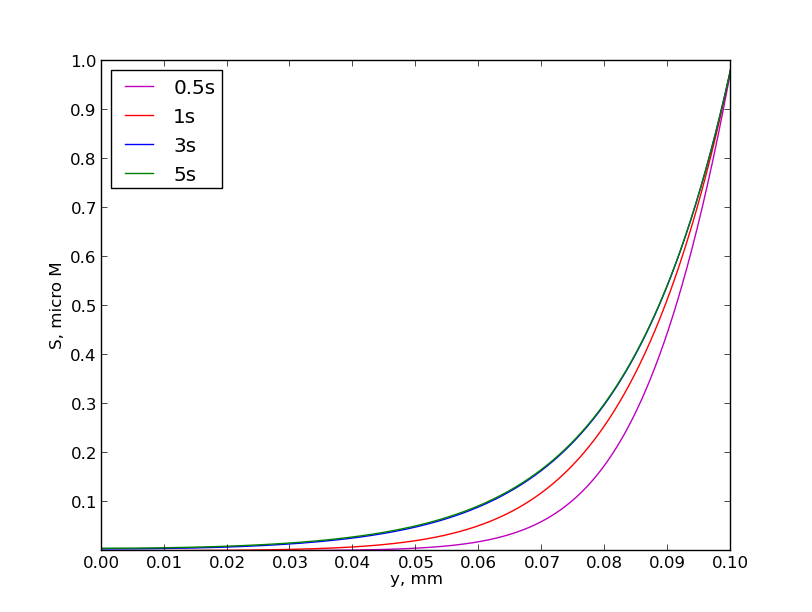
\includegraphics[scale=0.5]{img/kurS}
     \caption{Tiriamo mišinio veikliosios medžiagos (S) koncentracija
     $\Omega_2$ srityje.}
     \label{img:S}
 \end{figure}

Iš grafiko matosi, kad su nusistatytais parametrų dydžiais, jau trečią sekundę
pasiekta įsisotinusi (S) koncentracija fermento sluoksnyje. Erdvės taškas $y = 0$
atitinka biojutiklio ribą $x = d_0$, o erdvės taškas $y = 0.1$ atitinka
biojutiklio ribą $x = d_1$.

Apskaičiavus (S) koncentraciją visuose fermento sluoksnio erdvės žingsniuose ir
visuose nusistatyto laiko intervalo žingsniuose, remiantis rezulatais ir lygčių
sistema (\ref{eq:P}) galima apskaičiuoti reakcijos produkto (P) koncentraciją
selektyviosios membranos ir fermento sluoksniuose skirtingais laiko momentais.
Paveiksle (\ref{img:P}) yra pavaizduota dalis programos atliktų skaičiavimų,
t.y. reakcijos produkto (P) koncentracija selektyviosios ir
fermento membranų sluoksniuose, kurių atitinkami storiai yra $0.02$mm ir $0.1$mm, keturiais laiko momentais: $0.5$, $1$,
$3$ ir $5$ sekundės nuo simuliacijos pradžios.
 \begin{figure}[H]
     \centering
     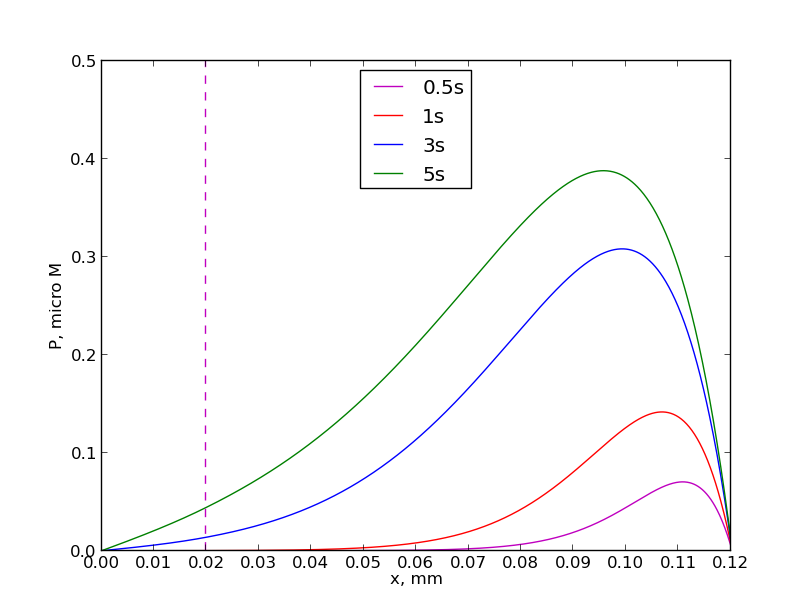
\includegraphics[scale=0.5]{img/kurP}
     \caption{Reakcijos produkto (P) koncentracija $\Omega_1$ ir $\Omega_2$
     srityse.}
     \label{img:P}
 \end{figure}
 
 Grafiko intervalas iki punktyrinės linijos $x\in(0 ;0.02)$ atitinka $\Omega_1$
 sritį, o už punktyrinės linijos $x\in(0.02;1.2)$ – $\Omega_2$ sritį. Praėjus penkioms sekundėms nuo simuliacijos pražios
 nėra pasiekta (P) įsisotinimo būsena stebimoje sistemoje.
 
 Apskaičiavus reakcijos produkto koncentraciją elektrodo paviršiuje ($x 
 \to 0$) nusistatyto laiko intervalo visais žingsniais ir remiantis formule
 (\ref{eq:i-form}) galima apskaičiuoti biojutiklio srovę tais laiko momentais.
 Paveiksle (\ref{img:I}) pavaizduota keturių biojutiklių su tuo pačiu
 selektyviosios membranos storiu, bet skirtingais fermento sluoksnio storiais,
 srovės dydžio priklausomybė nuo laiko atlikus simuliaciją su nusistatytais
 parametrų dydžiais.
 \begin{figure}[H]
     \centering
     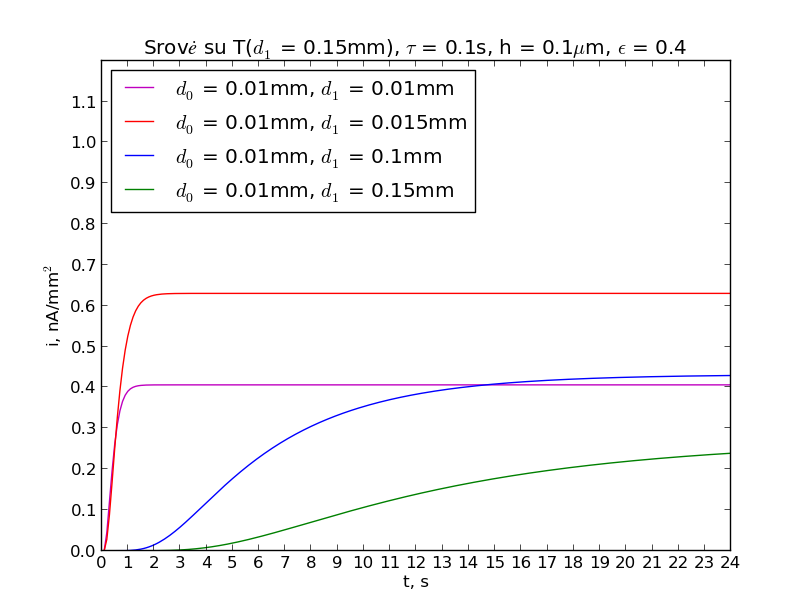
\includegraphics[scale=0.5]{img/kurI}
     \caption{Srovė, kai $\Omega_1 \in (0; d_0)$ ir $\Omega_2 \in (d_0; d_1)$.}
     \label{img:I}
 \end{figure}

 Remiantis srovės grafiku galima daryti išvadas, kad prie mažesnio storio
 sluoksnių srovė įsisotina greičiau ir kad selektyviajai membranai storėjant
 mažėja soties srovė, bet prie didesnio storio fermento membranų lėčiau.

\sectionnonum{Rezultatai ir išvados} 

Šiame darbe buvo pritaikyta amperometrinio biojutiklio su fermento sluoksniu
matematinis modelis ir jo atsako charakteristikos biojutikliui su selektyviaja
membrana. Tuo remiantis sudarytos matematinio modelio aproksimavimo lygtys, iš
kurių išvestos skaitinio sprendimo lygčių sistemos, ir susimuliuotas
biojutiklio veikimas naudojantis programa, kuri buvo sukurta remiantis
sudarytomis lygtimis.

Palyginus gautus grafikus su pateiktais \cite{baronas2003influence} ir
\cite{baronas2009mathematical} amperometrinių
biojutiklių grafikais galima daryti
išvadą, kad skaičiavimai yra neiškraipyti ir teisingi, ir kad 
pateikta programa sugeba atlikti 
korektiškus skaičiavimus. Ją galima panaudoti detalesniam tyrimui aiškintis selektyvios membranos
įtaką biojutiklio atsakui. Šiek tiek ją patobulinus galima apytiksliai
įvertinti optimalų vieno arba kito sluoksnio storį pagal apsibrėžtus parametrų
dydžius.

Šis darbas turi kelias tobulinimo kryptis. Viena iš jų būtų naudojantis turima
programa tirti kokie selektyvios membranos sluoksniai biojutikliams
turi didžiausią įtaką, pagal kriterijus įvertinti optimalų jos storį. Kita
kryptis būtų tobulinti patį modelį ir programą, kad jie tenkintų papildomas
sąlygas kaip (S) arba (P) perteklius prie elektrodo arba selektyvios membranos,
arba netolydus(nutrūkstamas) reakcijos produkto grafikas perėjime tarp
membranų. 

%\appendix
 
% \begin{figure}[H]
%     \centering
%     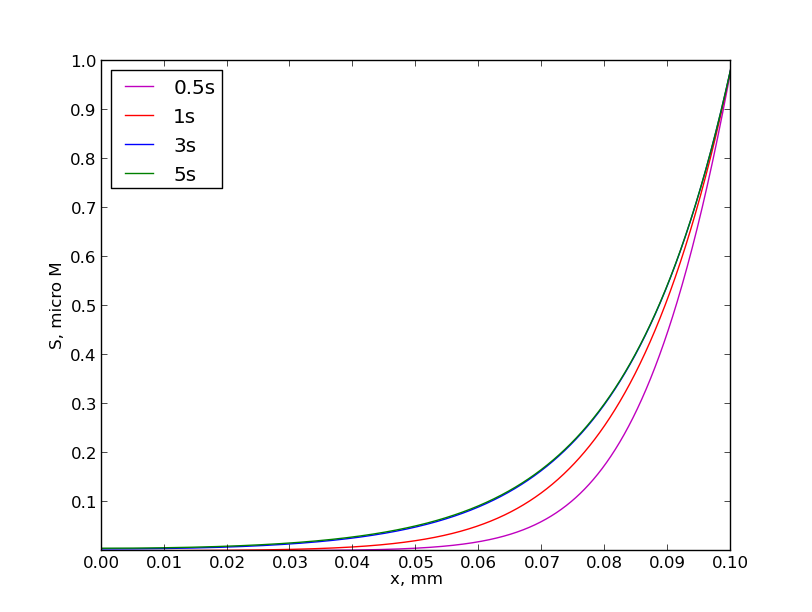
\includegraphics[scale=0.5]{img/S}
%     \caption{Substrate}
%     \label{img:mlp}
% \end{figure}
% 
% \begin{figure}[H]
%     \centering
%     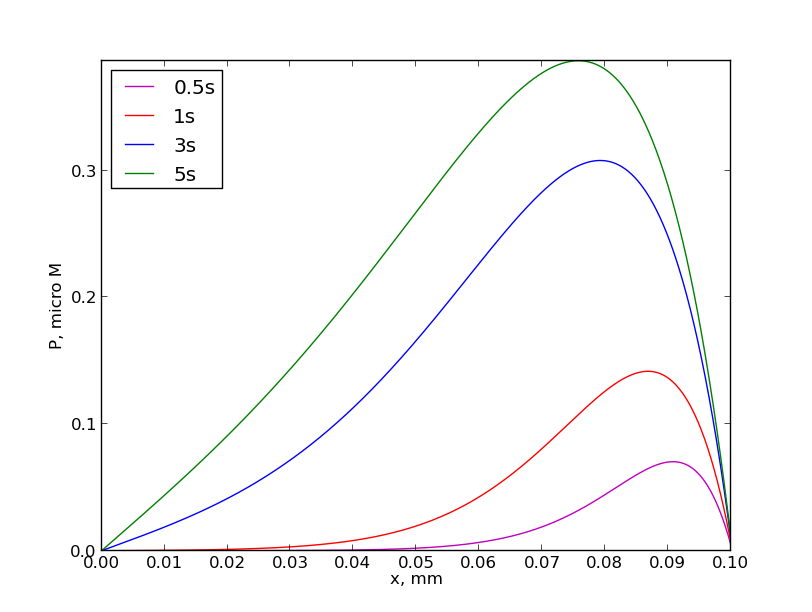
\includegraphics[scale=0.5]{img/P}
%     \caption{Product}
%     \label{img:mlp}
% \end{figure}
% 
% \begin{figure}[H]
%     \centering
%     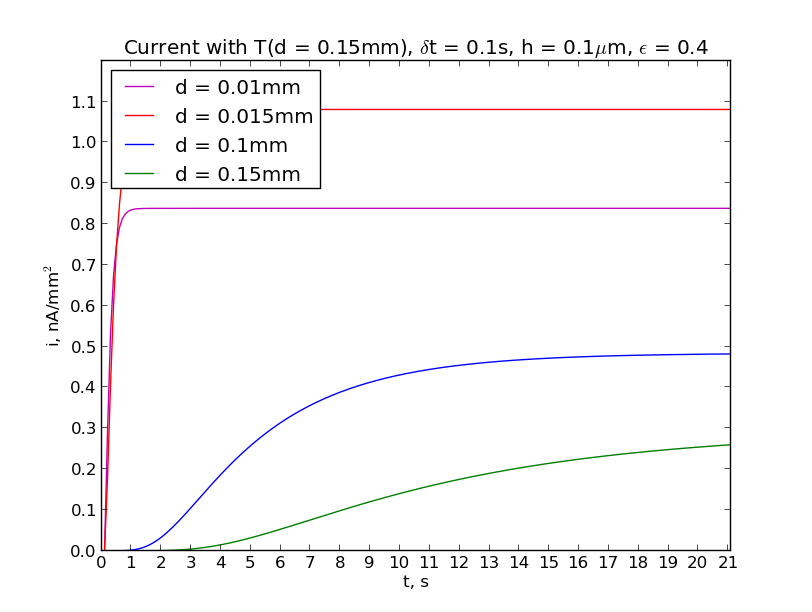
\includegraphics[scale=0.5]{img/i}
%     \caption{Current}
%     \label{img:mlp}
% \end{figure}
% 
%\appendix
%----------------------------------------------------

\bibliography{bibliografija}


\appendix

\section{Biojutiklio veikimo simuliacijos programa}
\label{programa}
Python yra aukšto lygio, efektyvi, nemokama ir patogi programavimo kalba.
Be to su šia programavimo kalba išeina naudoti matricų programavimo paradigmą,
kitaip tariant, Python turi Numpy biblioteką, kuri yra atviro kodo Matlab
atitikmuo. Tai reiškia, kad išeina patogiai atlikti veiksmus su matricomis.
Šioje programoje Numpy buvo panaudota elementų išrinkimui iš matricos,
konkrečiau (P) koncentracijos vertėms elektrodo paviršiuje.

\begin{verbatim}
# Programa parasyta su python programavimo kalba.
# Autorius Kestutis Gimbutas

# coding: utf-8
from matplotlib import pyplot as plt
from numpy import array, arange

def print_matrix(matrix):
    ''' Funkcija skirta sudarytu matricu spauzdinimui, naudota tikrinimui ir
    testavimui
    '''
    print 'micro m: ',
    for j in range(len(matrix[0])):
        print str(j*h)+ '    ',
    print
    for i, row in enumerate(matrix):
        print str(i*tau)+'s', ' '.join(['%.4f' % e for e in row])

def draw_matrix(substrate, n, label='S, micro M'):
    ''' Funkcija skirta nubraizyti substrato bei produkto koncentracijų grafikus'''
    x = [i*h/1000. for i in range(n)]
    plt.xlabel('x, mm')                 #braizant (P) grafika x pakeista i y
    plt.ylabel(label)
    plt.xticks(arange(min(x), max(x)+ (0.01), 0.01))
    plt.yticks(arange(0, 1 + 0.1, 0.1))
    plt.plot(x, substrate[int(0.5/tau)], 'm')
    plt.plot(x, substrate[int(1/tau)], 'r')
    plt.plot(x, substrate[int(3/tau)], 'b')
    plt.plot(x, substrate[int(5/tau - 1)], 'g')
    plt.legend(['0.5s','1s','3s','5s'],loc = 'left')

def get_current(product):
    '''Funkcija, kuri apskaičiuoja elektros srovę pagal pateiktą (P) verčių ant
    elektro paviršiau masyvą.
    '''
    return ne*F*Dp*array(product)/h/10**6

def draw_current(product, response_time, label, color):
    '''Funkcija skirta srovės grafikui nubraižyti'''
    time = [tau * i for i in range(int(response_time/h))]
    plt.xlabel('t, s')
    plt.ylabel(label)
    plt.xticks(arange(min(time), max(time)+ (0.01), 1))
    plt.yticks(arange(0, 1.2 + 0.1, 0.1))
    plt.plot(time, get_current(array(product)[0:int(response_time/tau), 1]), color)
    legend = []
    for k in range(4):
        legend.append('$d_0$ = ' + str(d0lengs[0]/1000.) + 'mm'+ ', $d_1$ = '
                                + str((d1lengs[k]+d0lengs[0])/1000.)+'mm')
    plt.legend(legend, loc = 'upper left')
    plt.title(u'Srov$ė$ su' + r' T($d_1$ = 0.17mm), $\mathbf{\tau}$ = 0.1s, 
                                h = 0.1$\mu$m, $\epsilon$ = 0.4')

def perkelties_metodas(coef):
    '''Funkcija skirta apskaiciuoti (S) ir (P) koncentracijas viename laiko
    zingsnyje, kaip parametras pateikiamas lygciu sistemos koeficientu rinkinys
    tame laiko zingsnyje
    '''
    CD = []
    for i in range(len(coef)):
        if i == 0:
            C1 = -coef[i][1] / coef[i][0]
            D1 = coef[i][2] / coef[i][0]
            CD.append([C1, D1])
        else:
            Ci = -(coef[i][2]/(coef[i][1] + (CD[-1][0] * coef[i][0])))
            Di = (coef[i][3] - (CD[-1][1] * coef[i][0])) / (coef[i][1]+(CD[-1][0] * coef[i][0]))
            CD.append([Ci, Di])
    Xn = CD[-1][1]
    X = [Xn]
    for j in range(len(coef)-2, -1, -1):
        Xi = CD[j][0] * X[-1] + CD[j][1]
        X.append(Xi)
    X.reverse()
    return X

# Apsibrėžti kintamieji    
S0 = 1                                      # 1 microM = 0,01KM
P0 = 0 
ne = 2
F = 96485                                   # Faradėjaus konstanta
Ds = 300                                    # 300 micro m^2/s
Dp = 300                                    # 300 micro m^2/s D2p
D1p = 100                                   # (P) ir selektyvios membranos koef
h = 0.1                                     # x erdves zingsnis x in [0;d1]
Km = 100                                    # 100 microM
Vmax = 100                                  # 100 microM/s
tau = 0.1                                   # delta zingsnio laikas
T = 50                                      # maksimalus stebejimo laikas
m = int(T / tau)                            # laiko zingsniu skaicius
epsilon = 0.40

def get_substrate_matrix():
    '''Funkcija, kuri apskaičiuoja (S) koncentraciją visuose fermento sluoksnio
    zingsniose visais laiko zingsniais naudojantis "perkelties_metodas" funkcijoja
    '''
    substrate = []
    for i in range(m):                      # laiko zingsniai
        substrate.append([])
        for j in range(n1):                 # membranos zingsniai
            if i == 0:
                substrate[i].append(0)
            else:
                substrate[i].append(None)
            if j == (n1 - 1):
                substrate[i][j] = S0
        if i != 0:
            coef_c = (h * h) / (tau * Ds)
            coef = []
            b1 = -1 - coef_c
            c1 = 1
           # d1 = 0
            d1 = ((h * h) / (Ds * tau)) * (((Vmax * substrate[i-1][1] * tau) / 
                (Km + substrate[i-1][1])) - substrate[i-1][1])
            coef.append([b1,c1,d1])
            for l in range(1, n1 - 1):
                al = 1
                bl = -2 - coef_c
                cl = 1
                dl = ((h * h) / (Ds * tau)) * (((Vmax * substrate[i-1][l] * tau)
                    /(Km + substrate[i-1][l])) - substrate[i-1][l])
                coef.append([al, bl, cl, dl])
            an = 1
            bn = -2 - coef_c
            cn = 0
            dn = -S0
            coef.append([an, bn, cn, dn])

            X = perkelties_metodas(coef)
            substrate[i][0] = X[0]
            for k in range(1, n1 - 1):
                substrate[i][k] = X[k - 1]
    return substrate

def get_product_matrix(substrate):
    '''Funkcija, kuri apskaičiuoja (P) koncentraciją visuose fermento sluoksnio
    zingsniose visais laiko zingsniais naudojantis "perkelties_metodas"
    funkcijoja ir funkcijos "get_substrate_matrix" (S) rezultatais
    '''
    product = []
    for i in range(m):
        product.append([])
        for j in range(n):
            if i == 0:
                product[i].append(0)
            else:
                product[i].append(None)
            if j == (n - 1):
                product[i][j] = P0
        if i != 0:
            coef_c = (h * h) / (tau * Dp)
            coef = []
            b1 = -2 - coef_c
            c1 = 1
            d1 = -1 * ((h * h) / (D1p * tau)) * product[i-1][1]
            coef.append([b1,c1,d1])
            for l in range(1, n - 1):
                al = 1
                bl = -2 - coef_c
                cl = 1
                if l <= n0:
                    dl =-1 * ((h * h) / (Dp * tau)) *  product[i-1][l]
                if l > n0:
                    dl =-1 * ((h * h) / (Dp * tau)) * (((Vmax * substrate[i-1][l-n0] * tau)
                        /(Km + substrate[i-1][l-n0])) + product[i-1][l])
                coef.append([al, bl, cl, dl])
            an = 1
            bn = -2 - coef_c
            cn = 0
            dn = -P0
            coef.append([an, bn, cn, dn])

            X = perkelties_metodas(coef)
            product[i][0] = X[0]
            for k in range(1, n - 1):
                product[i][k] = X[k - 1]
    return product

def get_T(product, enzyme_width):
    '''Funkcija, kuri apskaičiuoja T remiantis apsibrėžtais kintamaisiais ir
    apskaičiuotomis (P) vertėmis funkcijoje "get_product_matrix"
    '''
    time = 0
    i1 = get_current(array(product)[:, 1])
    for t in range(int(T/tau)):
        if time == 0 and (t*tau) > 2:
            if ((t*tau)/i1[t])*abs((i1[t]-i1[t-1])/((t*tau)-((t-1)*tau))) < epsilon:
                time = t * tau              # t- laiko zingsnis
    return time

if __name__ == '__main__':
    '''Programos dalis, kurioje įgyvendinta logika: iškviečiamos reikiamos funkcijos
    su joms reikalingais ir korektiškais parametrais
    '''
    d1 = 100                                # fermento sluoksnis
    n1 = int(d1 / h + 1)
    d0 = 20                                 # selektyvios membranos sluoksnis
    n0 = int(d0 / h + 1)
    substrate = get_substrate_matrix()
    draw_matrix(substrate, n1, 'S, micro M')
    plt.show()
    n = n1 + n0
    product = get_product_matrix(substrate)
    draw_matrix(product, n, 'P, micro M')
    plt.plot([d0/1000., d0/1000.], [0, 0.5], 'm--')
    plt.show()
    colors = ['m','r','b','g']
    d1lengs = [10, 15, 100, 150]             # fermento sluoksniai
    d0lengs = [20]
    for i1, d1 in enumerate(d1lengs):
        for i0, d0 in enumerate(d0lengs):
            n0 = int(d0 / h + 1)             # erdves zingsniu skaicius selektyvioj membranoj
            n1 = int(d1 / h + 1)             # erdves zingsniu skaicius fermente
            n = n1 + n0
            substrate = get_substrate_matrix()
            product = get_product_matrix(substrate)
            draw_current(product, T, 'i, nA/mm$^2$', colors[i1])
    T_response = get_T(product, 50)
    plt.xlim(0, T_response)
    plt.ylim(0, 1.2)
    plt.show()
\end{verbatim}

%\section{Papildomų eksperimentų rezultatų lentelės}
%\begin{figure}[H]
%    \centering
%    \includegraphics[scale=0.5]{img/MLP}
%    \caption{Paveikslėlio pavyzdys}
%    \label{img:mlp}
%\end{figure}
%
\end{document}
